\documentclass[a4paper]{report}
\usepackage[fontsize=14pt]{fontsize}
\usepackage{amsmath}
\usepackage{fontspec}
\usepackage{graphicx}
\usepackage{sidecap}
\usepackage{wrapfig}
\usepackage{cleveref}
\sidecaptionvpos{figure}{c}
\usepackage[english,ukrainian]{babel}

\setsansfont{CMU Sans Serif}
\setmainfont{CMU Serif}
\setmonofont{CMU Typewriter Text}
\defaultfontfeatures{Ligatures={TeX}}
\usepackage[math-style=TeX]{unicode-math}
\usepackage[footskip=1cm, headsep=0.3cm, left=2cm, top=2cm, right=2cm, bottom=2cm]{geometry}


\begin{document}
\pagestyle{empty}
    Дональд Ервін Кнут (рис. \ref{fig:knuth}) (10 січня 1938 , Мілвокі, Вісконсин ) --- інформатик, ідеолог програмування та почесний професор 
    Стенфордського університету. Автор фундаментальної праці \textit{«Мистецтво програмування»}; вважається одним з батьків аналізу 
    складності алгоритмів. Розробник
    \begin{wrapfigure}{l}{0.41\textwidth}
        \vspace{-15pt}
        \centering
        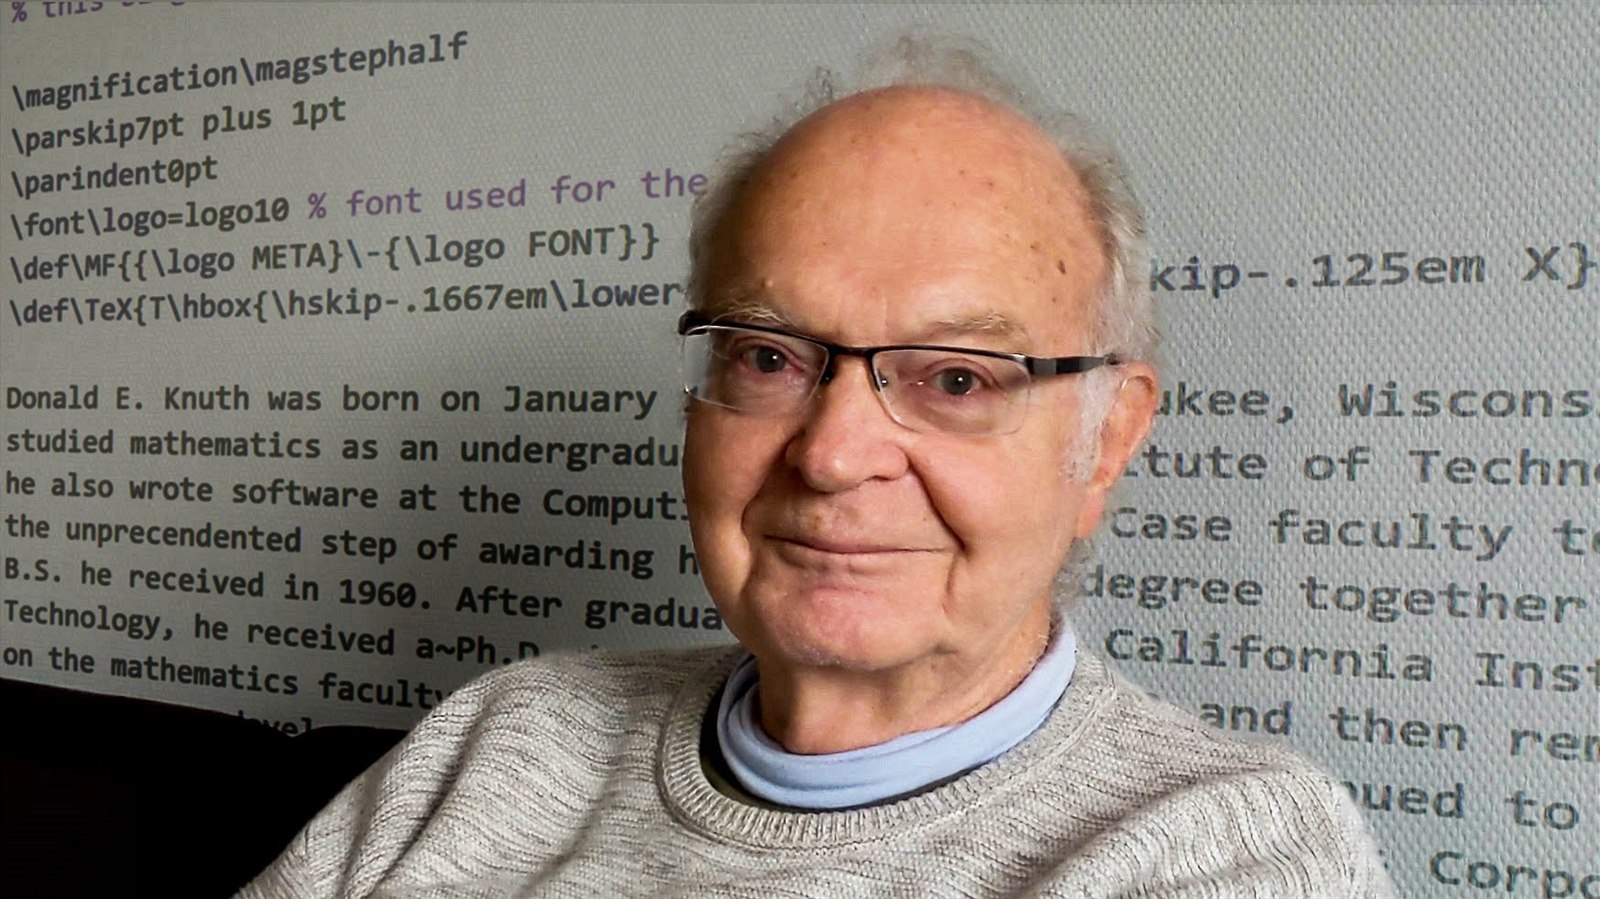
\includegraphics[width=0.41\textwidth]{Pictures/Knuth.jpeg}
        \caption{Дональд Ервін Кнут}
        \label{fig:knuth}
        \vspace{-15pt}
    \end{wrapfigure}
    типографічної системи \TeX{} та пов'язаної мови визначення шрифтів і системи їх рендерингу \texttt{METAFONT}.

    Кнут народився у місті Мілвокі, штат Вісконсин, в сім'ї німецьких американців Генрі Кнута та Луізи Марії Бонінг. 
    Батько Дональда працював на двох роботах: викладав бухгалетерію у Старшій Школі Мілвокі та вів невелике підприємство по друку. 
    Молодший Кнут, навчаючись у тій же школі, отримав багато академічних відзнак, більшість з яких за геніальні способи 
    вирішення різноманітних проблем. Наприклад, у восьмому класі він взяв участь у змаганні, в якому потрібно було відшукати 
    всі слова, які можна скласти з букв словосполуки «Ziegler's Giant Bar». У суддейському списку було 2500 слів, та Дональду 
    вдалось знайти 4500 та перемогти у конкурсі.

    Освіта У 1956 році Кнут отримав запрошення до Технологічного Інституту (рис. \ref{fig:CWRU}) у Клівленді, Огайо, де вперше познайомився з \texttt{IBM} 650, одним 
    із перших мейнфреймів. Прочитавши посібник до комп'ютера, Кнут вирішив переписати код компілятора для комп'ютера з його колишньої школи, тому що
    він вірив, що зможе зробити його краще.

    \begin{SCfigure}[0.5][h]
        \centering
        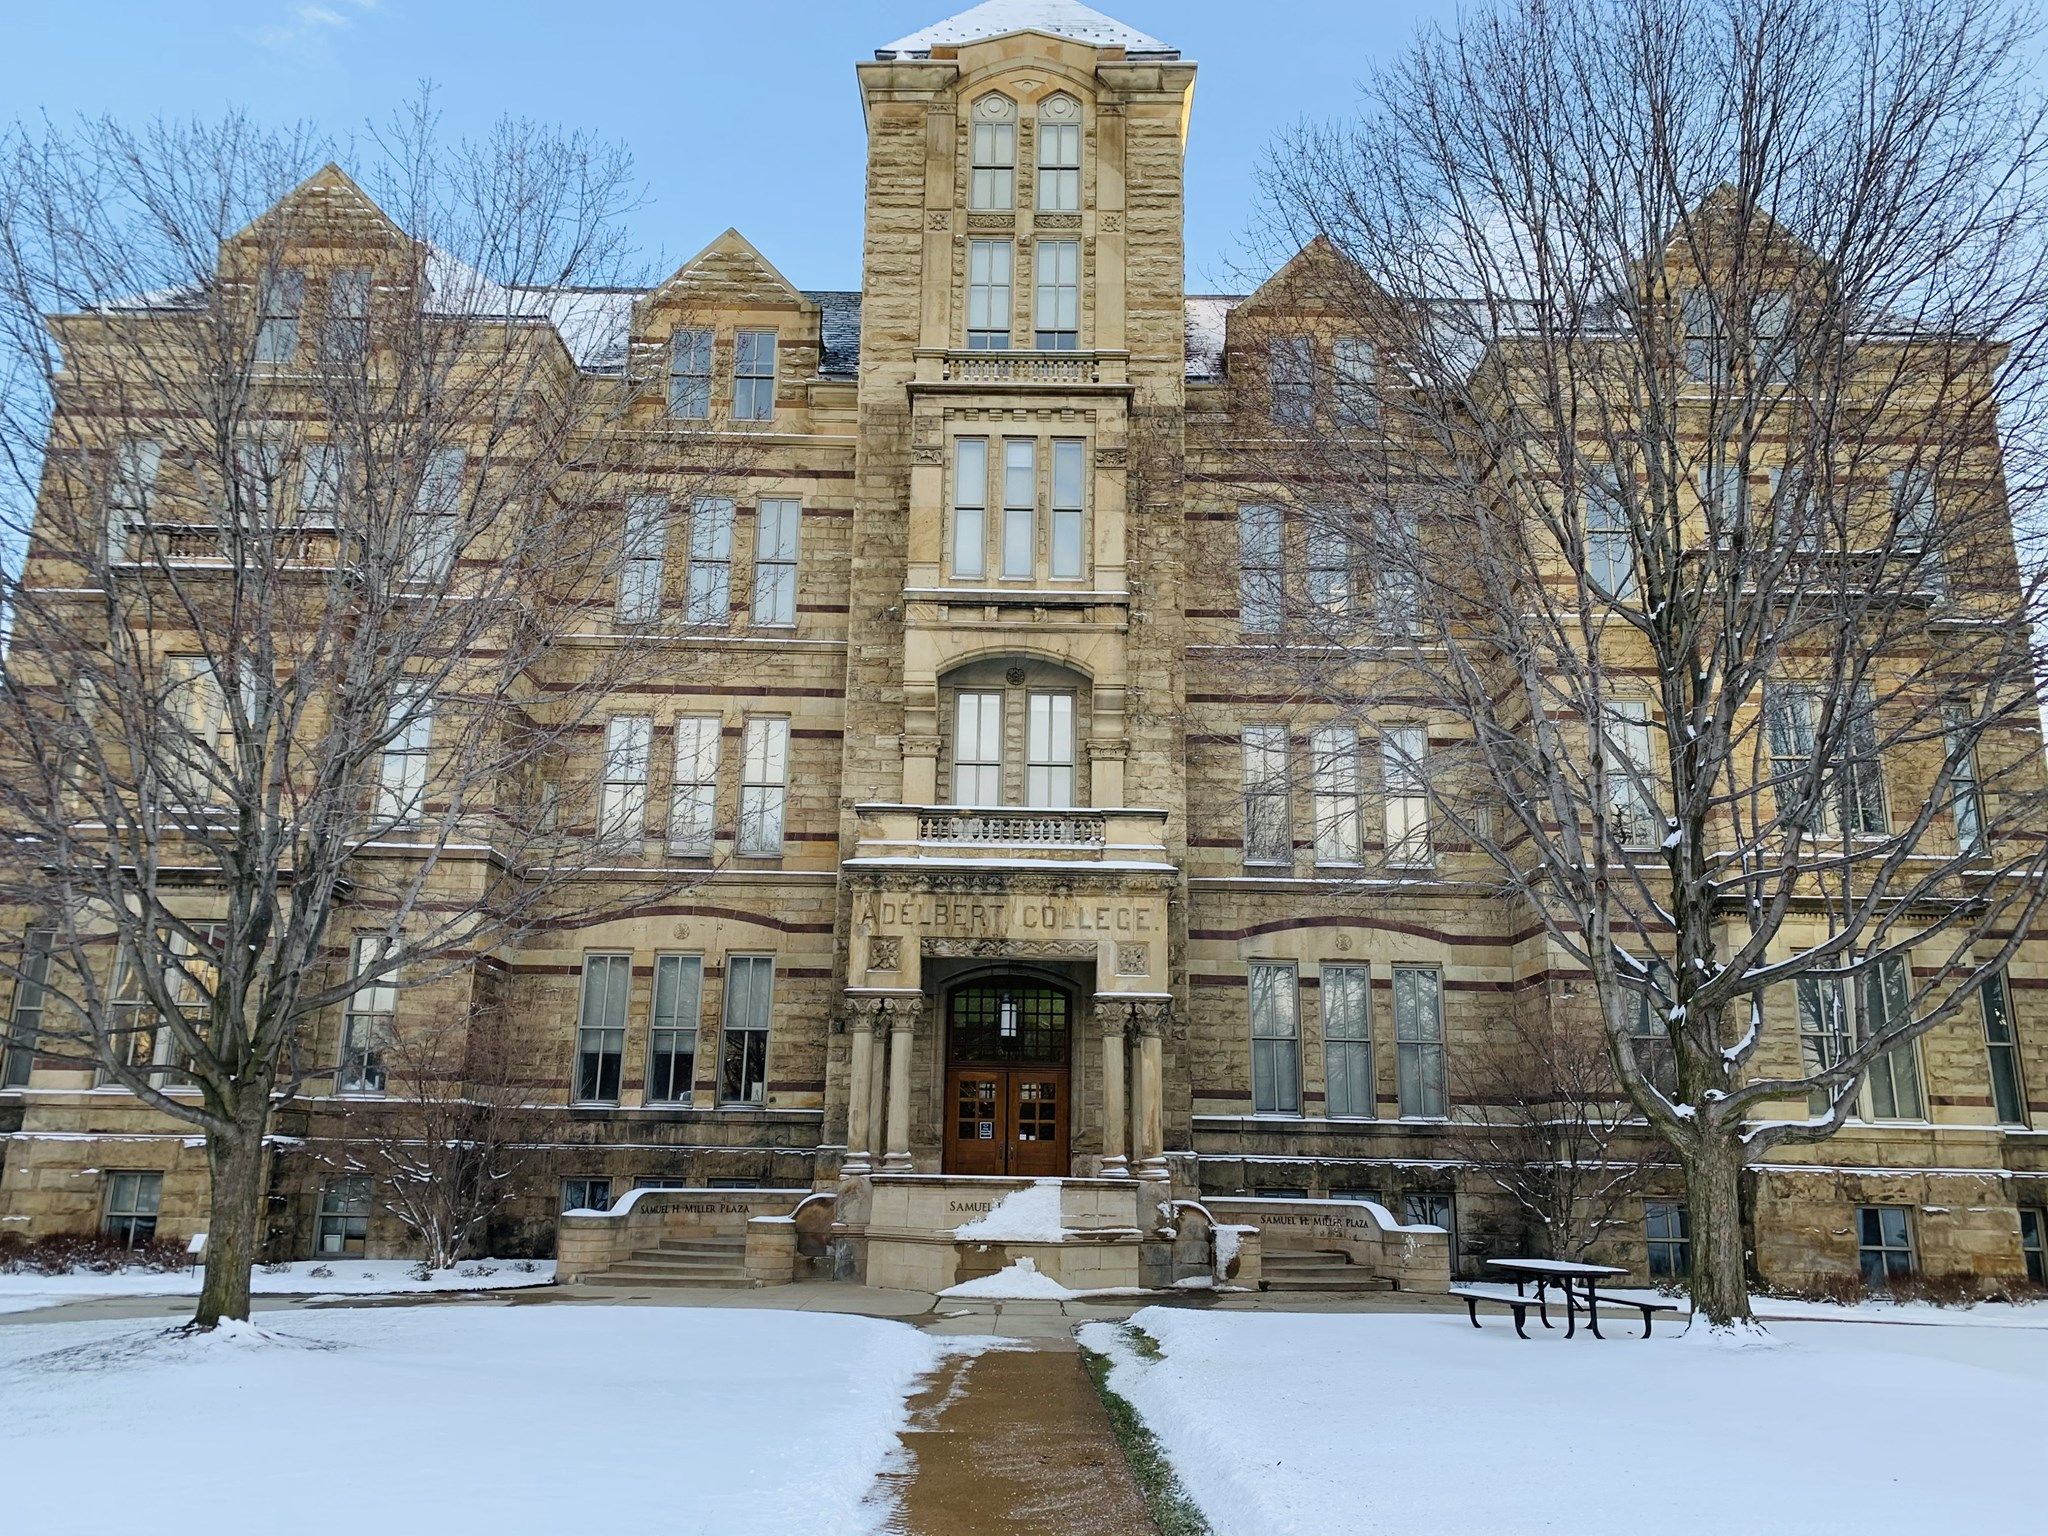
\includegraphics[width=0.6\textwidth]{Pictures/CWRU.jpg}
        \caption{Західний резервний університет Кейса (CWRU)}
        \label{fig:CWRU}
    \end{SCfigure}

    У 1958 році Кнут створив програму, щоб допомогти шкільній баскетбольній команді вигравати більше матчів. Він призначив кожному гравцю
    «вартість», щоб оцінити імовірність кожного баскетболіста здобути очки. Цей підхід оцінили видання Newsweek і CBS Evening News, згадавши Кнута
    у своїх випусках.
    
\end{document}